%% Preamble
% Document type, packages imported, theme and color:
\documentclass{beamer}
\usepackage{amsmath,geometry,graphicx}
\usepackage{tcolorbox}
\usetheme{Madrid}
\usepackage{multicol}
\newcommand{\BRDF}{\mathrm{BRDF}}
\newcommand{\MRDF}{\mathrm{MRDF}}
\newcommand{\ip}[2]{\langle {#1}, {#2} \rangle}

% Title page
\title{Semi-analytical BRDF-based quantification of light reflection}

\date{July 25, 2018}
\author{
Michael Byrne, 
Fatoumata Sanogo,
Pai Song,
Kevin Tsai,
Hang Yang, and
Li Zhu\\
\medskip
Problem Presenter:  John Peach (MIT Lincoln Lab)\\
Faculty Mentor: Alen Alexanderian (NCSU)
}
\titlegraphic{}
\institute[Abbreviation]{SAMSI-IMSM}

%% Presentation
\begin{document}

\begin{frame}
\titlepage
\end{frame}

\begin{frame}[t] 
\frametitle{Motivation} 
\begin{itemize} 
\item Satellite tracking 
\item Prediction of reflective response 
\item Guide model calibration 
\vspace{2mm}
\end{itemize} 
\centerline{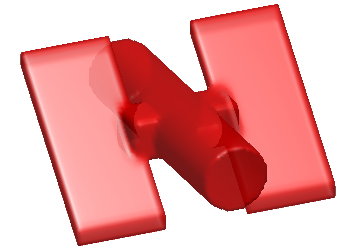
\includegraphics[width = 0.5\linewidth]{./figs/Satellite.jpg}} 
\end{frame} 
 
\begin{frame}[t]
\frametitle{Goals} 

\begin{columns}
\begin{column}{0.5\textwidth}
\begin{itemize} 
\item Build complex objects using various methods (OpenSCAD, R-functions) \vspace*{8mm}
\item Develop a continuous approach to optical cross section computation \vspace*{10mm}
\item Find a solution to the multi-path problem 
\end{itemize} 
\end{column}
\begin{column}{0.5\textwidth}
\vspace{5mm}
\centerline{\includegraphics[scale = 0.2]{rocket.pdf}}\\ 
\vspace{5mm}
\centerline{
\includegraphics[scale = 0.5]{./figs/icosahedron_single.pdf}}
\vspace{5mm}
\centerline{\includegraphics[scale = 0.15]{./figs/multipath.pdf}}
\end{column}
\end{columns}

\end{frame} 

\begin{frame}
\frametitle{OpenSCAD} 
\centerline{\includegraphics[scale = 0.35]{./figs/sdh_openscad}} 
\end{frame}

\begin{frame} 
\frametitle{Rvachev functions (1963)} 
\begin{itemize} 
\item Commonly referred to as R-functions 
\item Inputs are functions
\item ``Boolean algebra" on functional representation to construct composite shapes from simple ones. \\
Let $f,g$ be two functions and $f=0$ generate geometric object $A$ and $g=0$ generates geometric object $B$. Define 
\[
    \begin{aligned}
    f \land_0 g &= f + g + \sqrt{f^2 + g^2}       \\ 
    f \lor_0 g &= f + g - \sqrt{f^2 + g^2}       \\
    f \setminus_0 g &= f - g - \sqrt{f^2 + g^2}  \\
    \end{aligned}
\]
\end{itemize} 
\end{frame}
\begin{frame}[t] 
\frametitle{R-functions -- examples} 
Union of two spheres:
\[
   \begin{aligned}
   A&: f(x,y,z)=x^2+y^2+z^2 - 1 &= 0 \\
   B&: g(x,y,z)=\left(x-\frac{3}{2}\right)^2+y^2+z^2 - 1 &= 0 \\
   \end{aligned}
\]


\begin{center}
{\tiny
\centerline{\includegraphics[width = 0.75\linewidth]{./figs/TwoSpheres}} 
\vspace{-3mm}
$
A \cup B: {f\lor_0 g=0\Leftrightarrow \left(x-\frac{3}{2}\right)}^2-\sqrt{{\left(x^2+y^2+z^2-1\right)}^2+{\left({\left(x-\frac{3}{2}\right)}^2+y^2+z^2-1\right)}^2}+x^2+2\,y^2+2\,z^2-2 = 0$ 
}
\end{center}
\end{frame} 

\begin{frame}
\frametitle{R-functions -- examples} 
\centerline{\begin{tabular}{cc}
\includegraphics[width=.32\textwidth]{./figs/shape1.pdf} &
\includegraphics[width=.32\textwidth]{./figs/shape2.pdf}  
\\
$A$ & $B$
\end{tabular}}
\begin{tabular}{ccc}
\includegraphics[width=.32\textwidth]{./figs/union.pdf} & 
\includegraphics[width=.32\textwidth]{./figs/intersect.pdf} & 
\includegraphics[width=.32\textwidth]{./figs/diff.pdf}\\
$A \cup B$ & $A \cap B$ & $A \setminus B$ 
\end{tabular}
\end{frame} 

\begin{frame}[fragile]
\frametitle{Optical cross section (OCS)}
\begin{itemize}
\item Accumulate reflectance over a target surface
\item Discrete: Sum over triangular facets 
\item Continuous: Analytic formulas (use R-functions); 
used \verb+chebfun+ for computing integrals
\end{itemize}
\centerline{\includegraphics[scale = 0.5]{./figs/facet.png} \: \includegraphics[scale = 0.5]{./figs/icosahedron.png}}
\end{frame}

\begin{frame}[t]
\frametitle{The Blinn--Phong model}
\centerline{\includegraphics[scale=0.2]{./figs/ModelVectors}}
\begin{tcolorbox}
$$\text{BRDF}(\mathbf{I},\mathbf{V};\mathbf{N}) = \left(\frac{\langle\mathbf{H},\mathbf{N}\rangle}{\|\mathbf{H}\|}\right)^\alpha \text{ for } \alpha \geq 0$$
\centerline{where $\mathbf{H} = \mathbf{I} + \mathbf{V}$ is the \textit{halfway vector}}
\end{tcolorbox}
\begin{itemize}
\item Modification of Phong model
\item BRDF: \textit{Bi-static reflectance distribution function}
\end{itemize}
\end{frame}

\begin{frame}[t]
\frametitle{Blinn--Phong as MRDF}
\begin{itemize}
\item MRDF: \textit{Mono-static reflectance distribution function}
\item Case where light and viewing vectors are parallel
\item Blinn--Phong model reduces to $(\cos\theta)^\alpha$ \\
($\theta$ denotes the angle between viewing/light vectors and the surface normal)

%\vspace*{0.1 in} 
\end{itemize}
\centerline{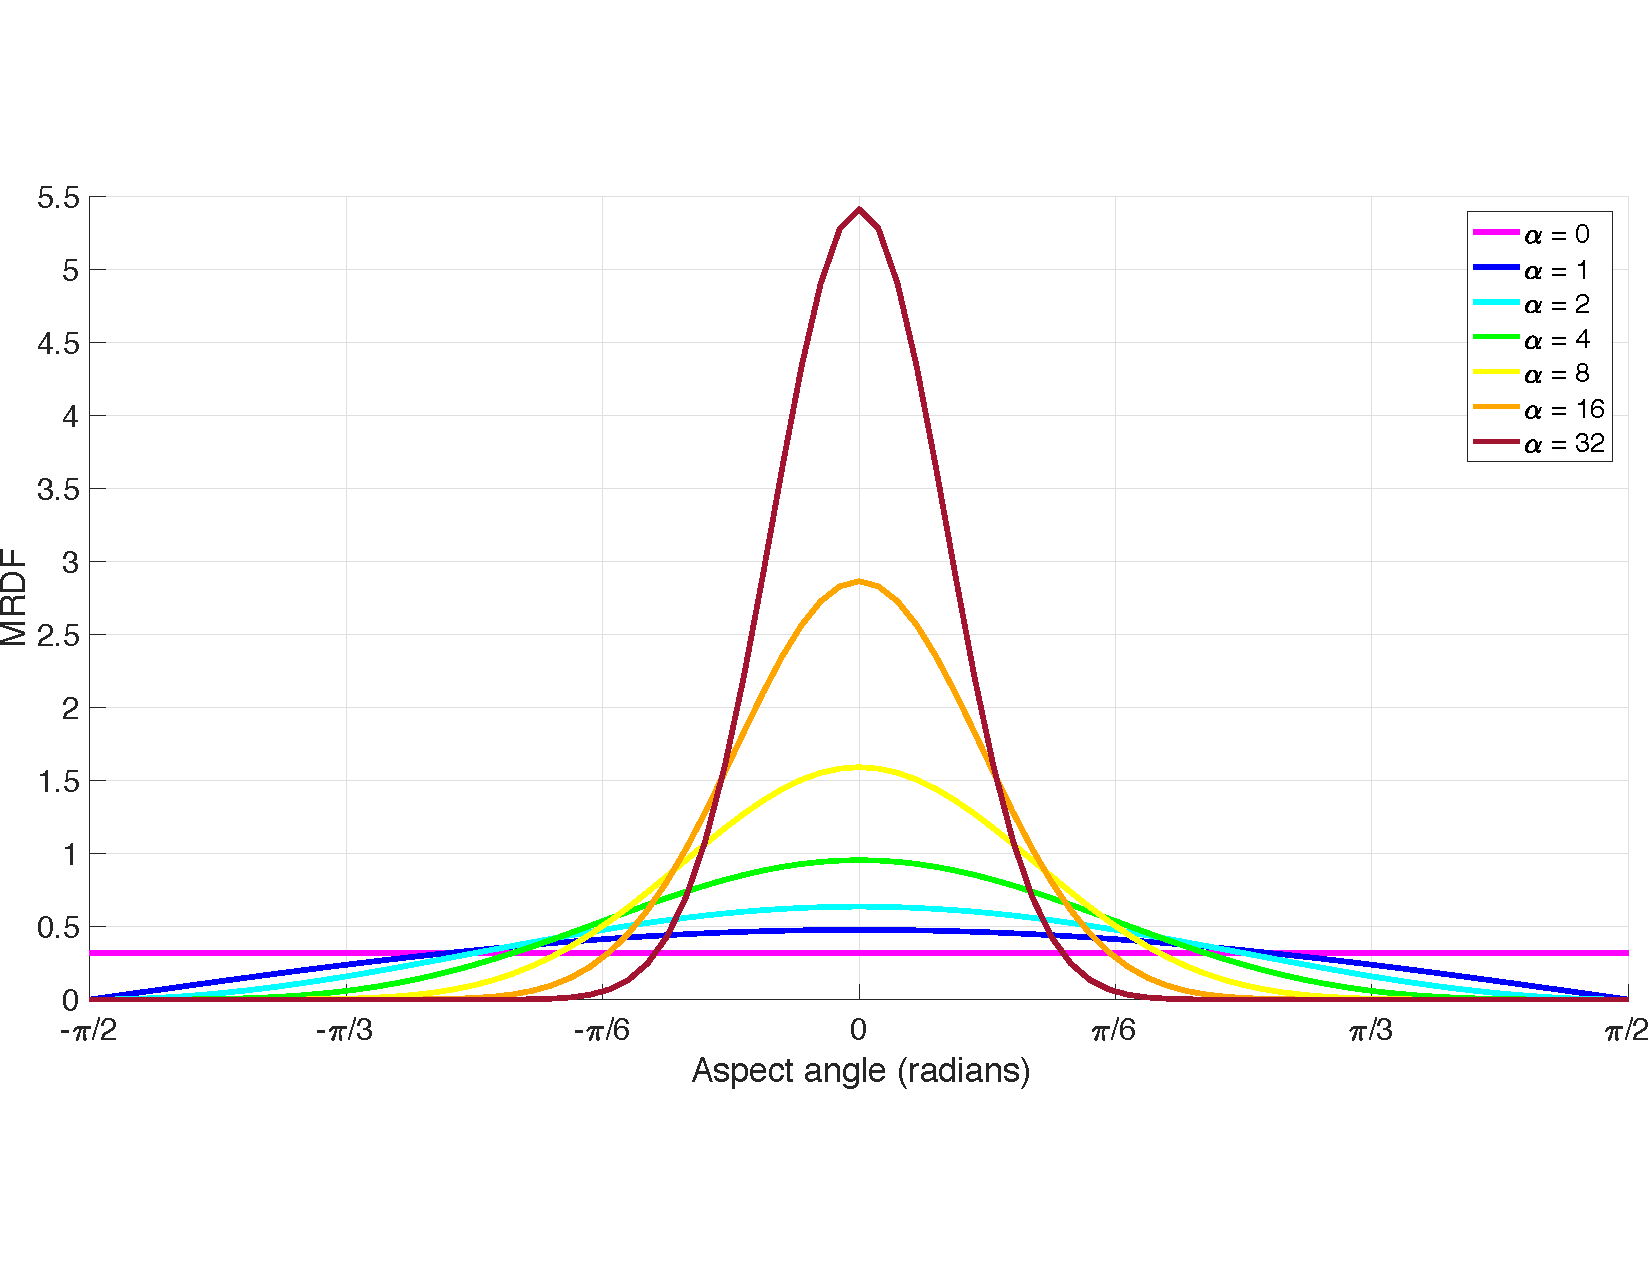
\includegraphics[scale=0.32]{./figs/MRDFs2}}
\end{frame}

\begin{frame}
\frametitle{Blinn--Phong as BRDF}
\centerline{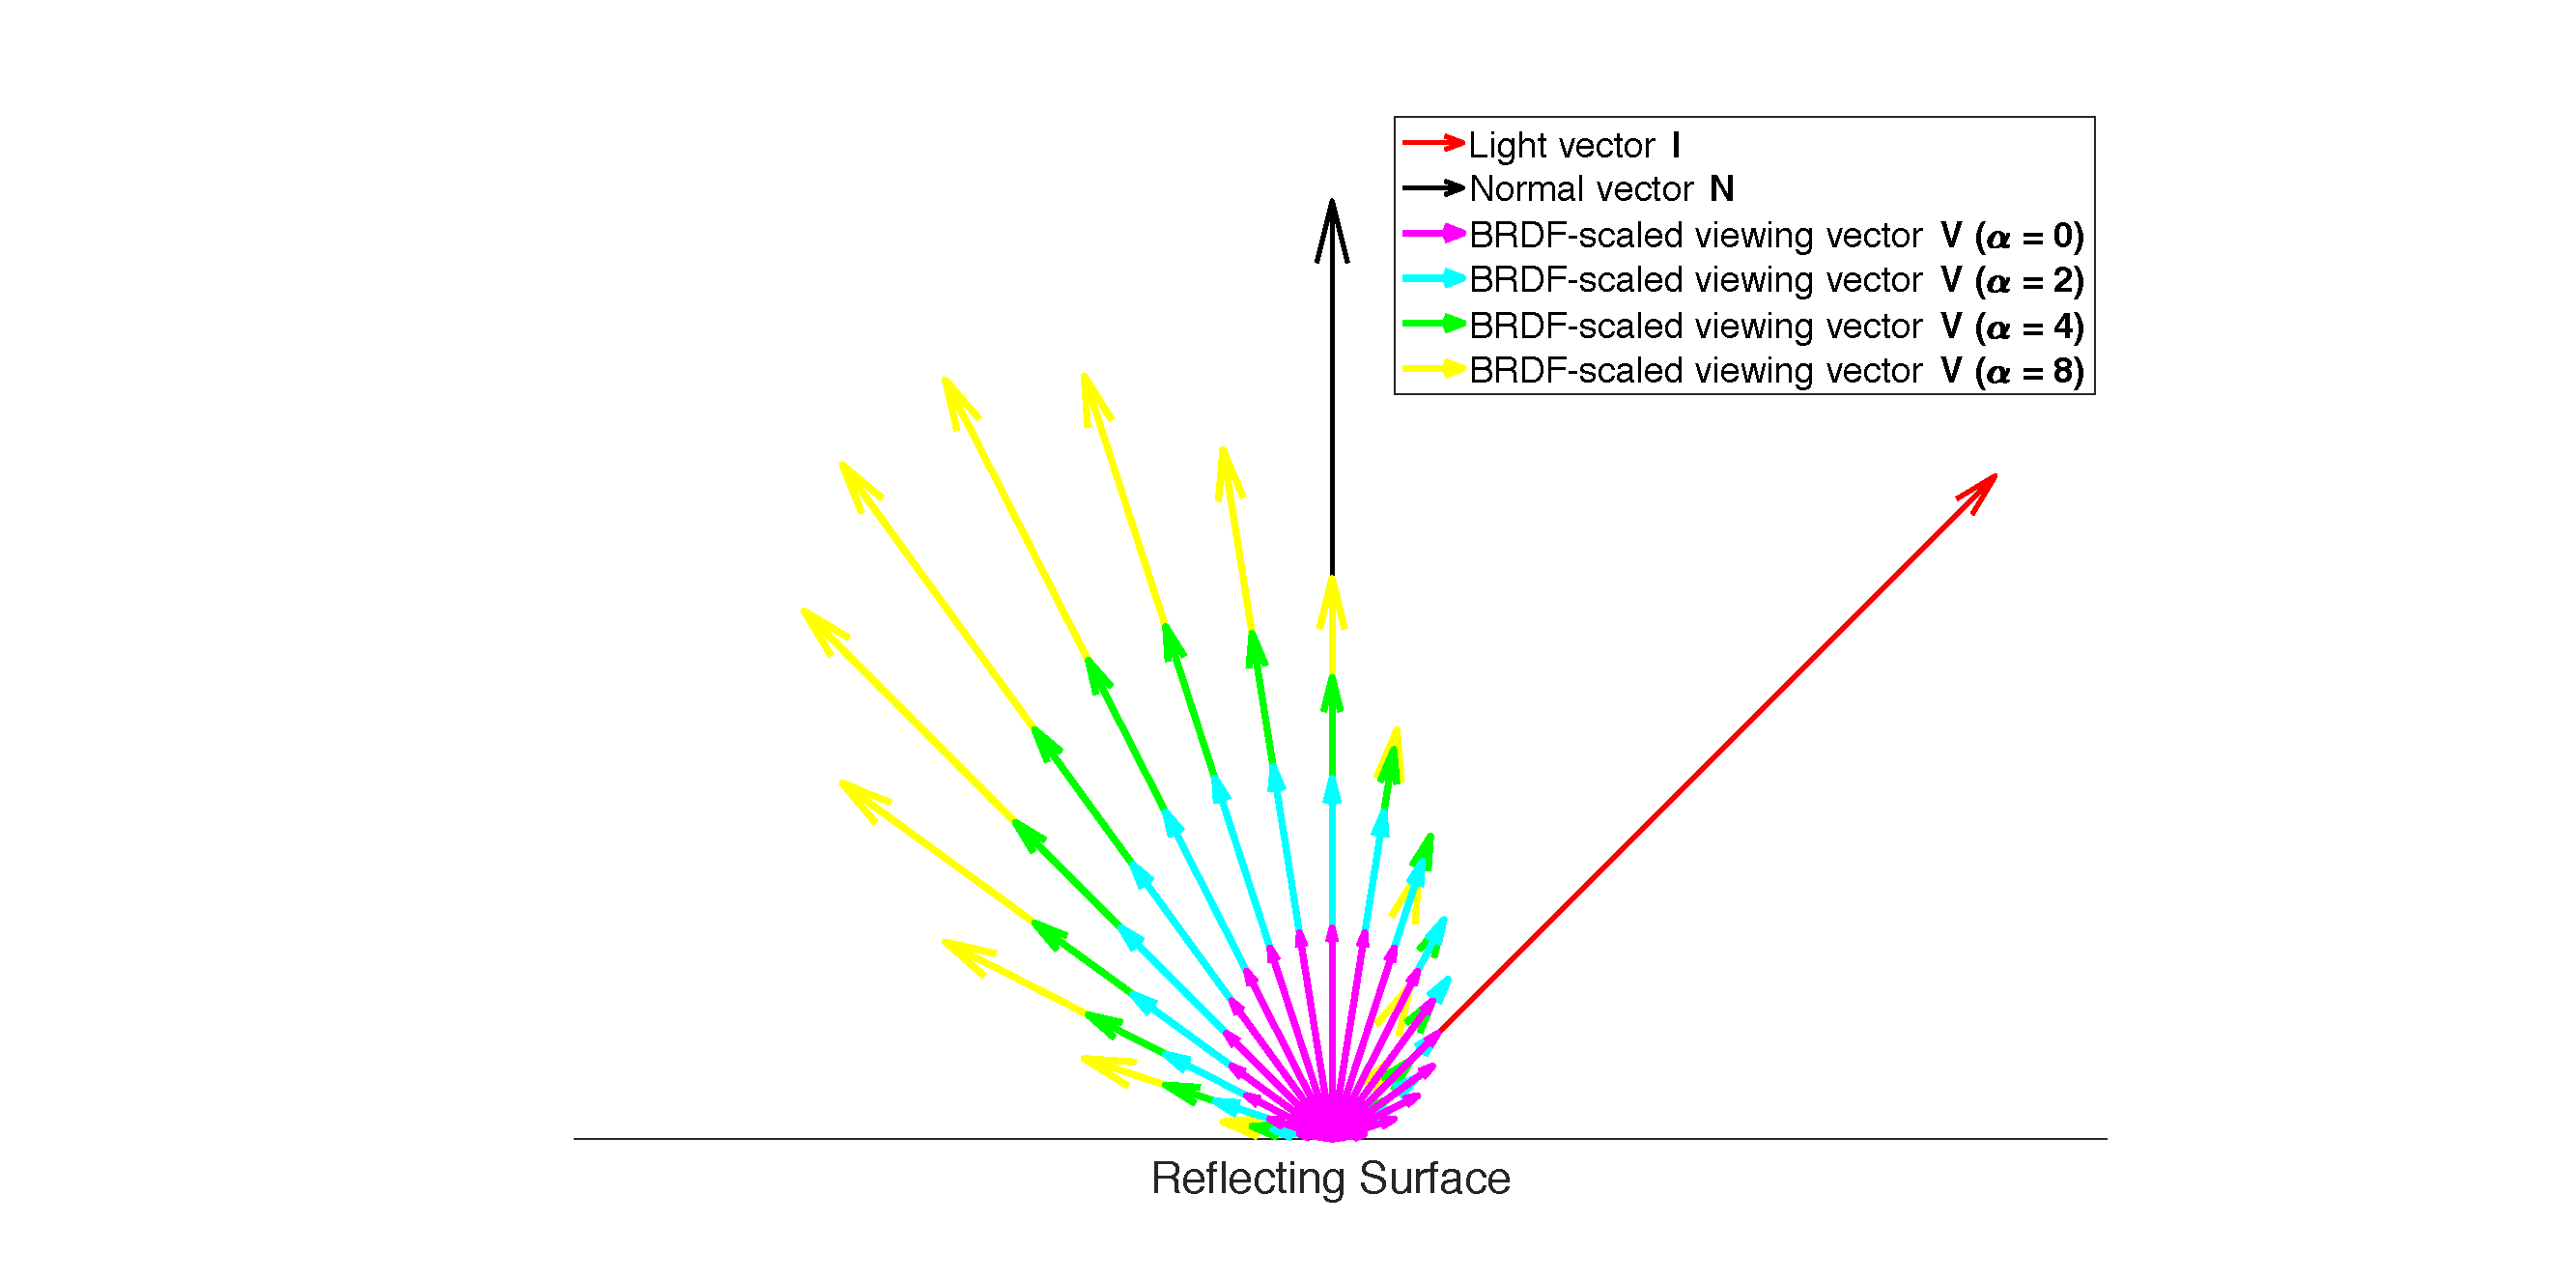
\includegraphics[scale=0.4]{./figs/BRDF_Vectors.pdf}}
\end{frame}

\begin{frame}[t]
\frametitle{Analytic benchmark: the sphere}
\begin{itemize}
\item (LEFT) Unit sphere, (RIGHT) Ellipsoid
\item Light source: fixed at the direction $(\theta,\phi) = (\frac{\pi}{2},\frac{\pi}{2})$
\item Detector: orbiting on $xy$-plane
\item Analytic solution for sphere: $2\pi/3 \approx 2.094395102393195$
\item Chebfun approximation for sphere: $\approx 2.094395102389723$
\end{itemize}
\begin{columns}[c]
\column{.5\textwidth}
\centering 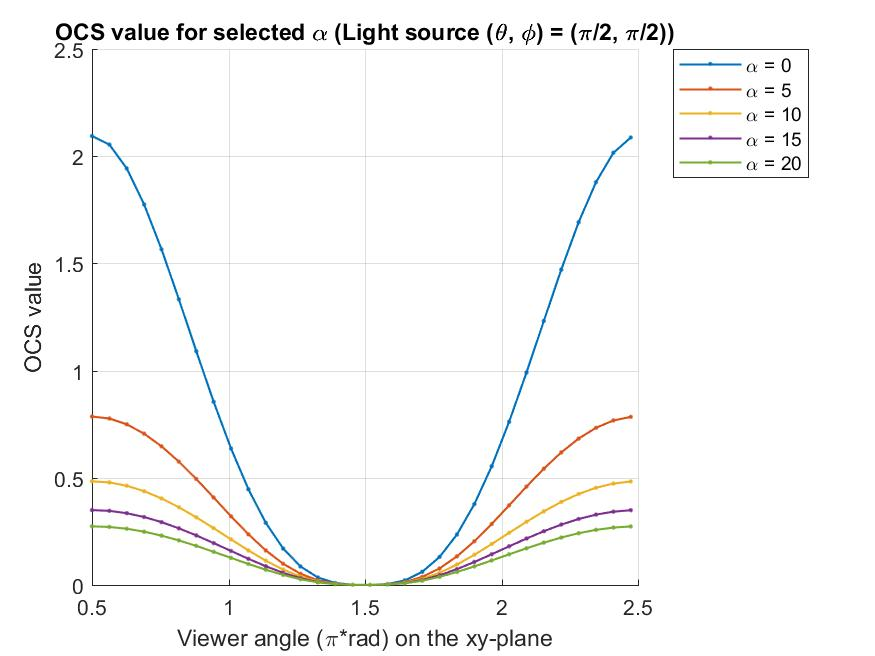
\includegraphics[scale=0.21]{./figs/OCS_parallel_plane}
\column{.5\textwidth}
\centering 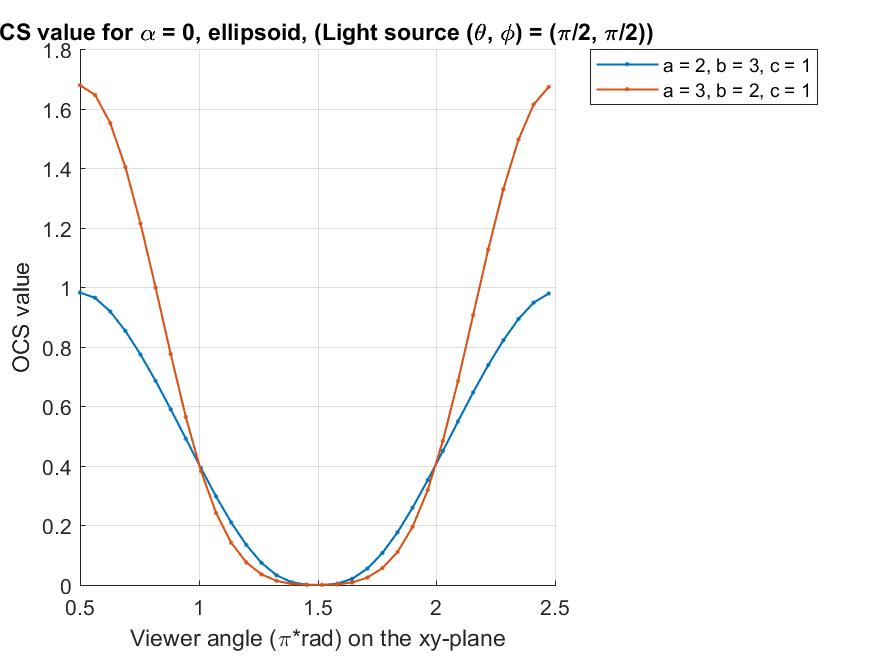
\includegraphics[scale=0.21]{./figs/OCS_parallel_plane_ellipsoid}
\end{columns}
\end{frame}

\begin{frame}[t]
\frametitle{Analytic benchmark: OCS values of sphere \& ellipsoid}
\begin{itemize}
\item (LEFT) Unit sphere, (RIGHT) Ellipsoid
\item Light source: fixed at the direction $(\theta,\phi) = (0,0)$
\item Detector: orbiting on $xy$-plane
\item Varying specular highlight
\end{itemize}
\begin{center}
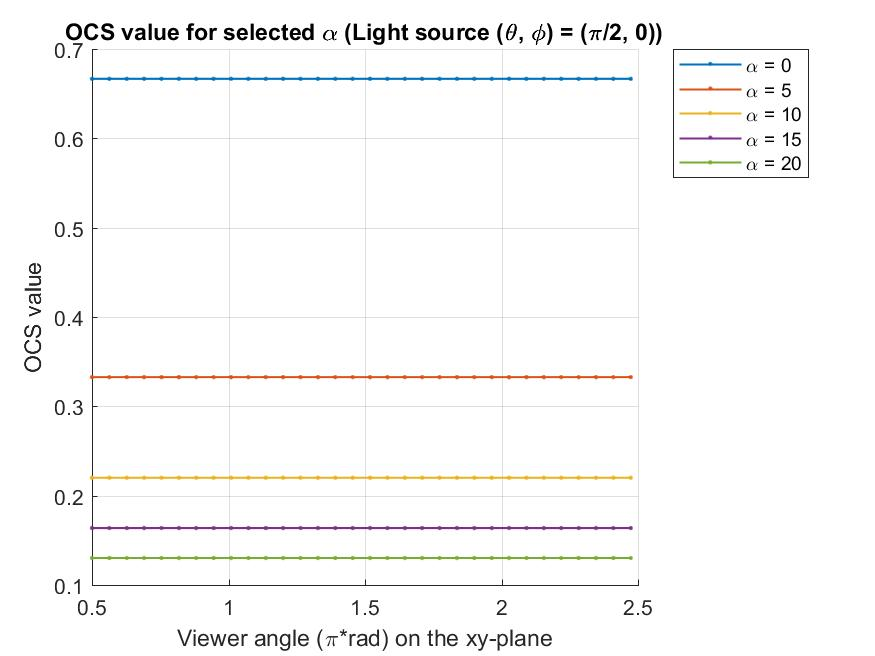
\includegraphics[width=.45\textwidth]{./figs/OCS_perpendicular_plane}
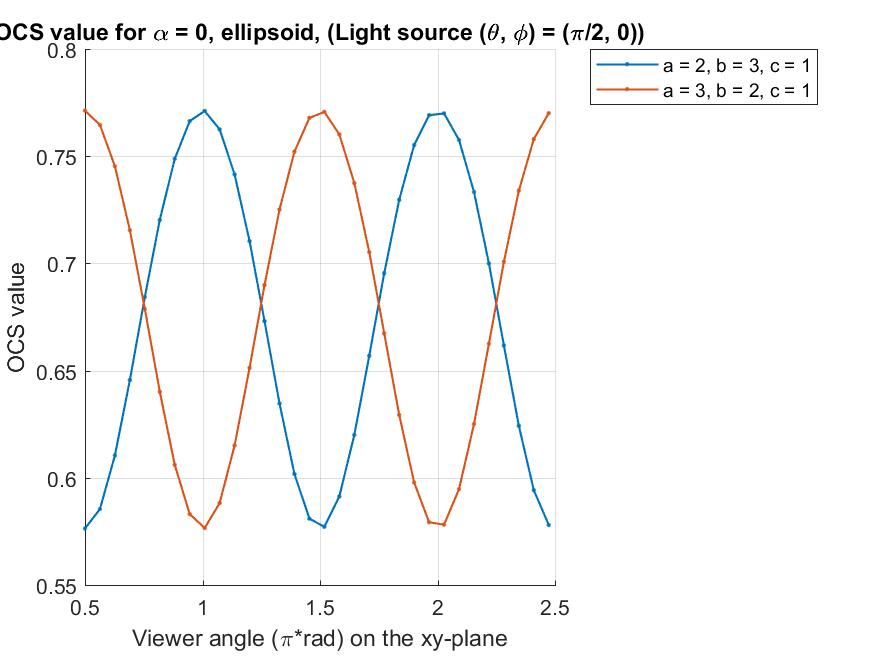
\includegraphics[width=.45\textwidth]{./figs/OCS_perpendicular_plane_ellipsoid}
\end{center}
\end{frame}


\begin{frame}[t]
\frametitle{Multi-path problem}
When light is projected onto a concave surface, some light beams could be reflected multiple times before it exits the surface area. 
\begin{columns}
\column{0.5 \textwidth} \includegraphics[width=2.4in]{./figs/multipath_edit.pdf}
\column{0.5 \textwidth} $N_i=(-\cos \theta_i,-\sin\theta_i)$\\ $I_i=(-\cos \psi_i,-\sin\psi_i)$\\ Plane geometry gives $\psi_{i}=\psi_{i-1}-\pi+\theta_i-\theta_{i-1}$
\end{columns}
Need to compute separately for each bouncing case. Denote contributions from lights that bounce exactly $n-$times before received by detector by $\sigma_n$.
\end{frame}

\begin{frame}[t]
\frametitle{Multi-path problem}
``Projected" $\BRDF$ at each bounce
$$\BRDF^*_{D_i}=\Bigg(\frac{\ip{\mathbf{I}_i+\mathbf{I}_{i+1}}{\mathbf{N}}}{\|\mathbf{I}_i+\mathbf{I}_{i+1}\|}\Bigg)^\alpha\frac{\ip{\mathbf{I}_i}{\mathbf{N}_i}}{\|\mathbf{I}_i\|\|\mathbf{N}_i\|}\frac{\ip{\mathbf{I}_{i+1}}{\mathbf{N}_i}}{\|\mathbf{I}_{i+1}\|\|\mathbf{N}_i\|} \frac{1}{\|r\mathbf{N}_{i+1}-r\mathbf{N}_i\|^2}$$
Contribution to OCS from lights that bounces exactly $n-$times 
\begin{equation*}
\sigma_n =\int_{0}^{\pi}...\int_{0}^{\pi}\BRDF(\mathbf{I}_n,\mathbf{V};\mathbf{N_n})\bigg(\prod_{i=1}^{n-1}\BRDF^*_{D_i}\bigg) |J|^n\mathrm{d}\vartheta_1...\mathrm{d}\vartheta_n , \quad |J|=r
\end{equation*}
Add up to get the whole OCS
$$\sigma=\sum_{n=1}^{\infty} \sigma_n$$
\end{frame}

\begin{frame}[t]
\frametitle{Conclusion}
\underline{Summary of results}:
\begin{itemize}
\item Implicit representations of composite objects readily obtained from R-functions 
\item Advantages of continuous OCS computation for simple shapes
\item Multi-path solution for semicircle interior
\end{itemize}
\underline{Future work}:
\begin{itemize}
\item Investigate continuous solutions for more complex/``sharper" objects 
\item Extend multi-path solution to interiors of other shapes
\end{itemize}
\centerline{
\includegraphics[scale=0.3]{./figs/Satellite.pdf}}
\end{frame}

\begin{frame}[t]
\frametitle{Image references}
\begin{itemize}
\item Satellite image from ``Motivation" frame: \\
https://www.newscientist.com/article/2113311-first-ever-lightning-mapping-satellite-set-for-take-off/ 
\item OpenSCAD image from ``OpenSCAD" frame: \\
http://sfepy.org/doc-devel/preprocessing.html
\item Vectors image from ``The Blinn--Phong model" frame is modified from original:
Martin Kraus - Own work, CC0, https://commons.wikimedia.org/w/index.php?curid=15534756
\end{itemize}
\end{frame}

\end{document}
